%!TEX root = ../report.tex
\chapter{Problem statement}

Digitalization of education is receiving close review nowadays. All over the world, including Germany, universities themselves and such organization as E-Assessment NRW (\url{http://www.eassessmentnrw.de/}) or Stifterverband (\url{https://www.stifterverband.org/}) put a lot of work into bringing innovations to the study process. Such learning management system as ILIAS (\url{www.ilias.de}), Moodle (\url{https://moodle.de/}), Blackboard (\url{http://de.blackboard.com}), Mahara (\url{https://mahara.org/}) and many others are used to make the process of education faster and easier for students as well as for teachers. Our university -- Hochschule Bonn-Rhein-Sieg (HBRS) -- uses ILIAS system for communication between students and professors, homework submission, providing feedback and testing. However, whereas ILIAS is widely used for homework submission and grading, it is not that popular for tests. The main reason is that the assessment types are significantly limited. In Table \ref{lea} one can see that except for Flash and Java Applet there are no programming assignments, and the ones with formulas are restricted to the very simple ones. Autograding of free texts is restricted to keywords spotting, while autograding of formulas can only be performed numerical substitution. It shows how important it is, to extend the types of autograded questions to programs, formulas and free text.\\

\begin{table}[]
\centering
\caption{ILIAS question types (\url{https://lea.hochschule-bonn-rhein-sieg.de/goto.php?target=wiki\_360501\_Welche\_Fragentypen\_gibt\_es\_und\_was\_mache\_ich\_damit\%3F})}
\label{lea}
\begin{tabular}{|l|l|l|}
\hline
Question type & Autogradability \\ \hline
single choice question  & autograded \\ \hline
multiple choice question & autograded \\ \hline
true/false question & autograded \\ \hline
mark a mistake question & autograded \\ \hline
hot spot/image map-question & autograded\\ \hline
fill the gap question & 	autograded\\ \hline
numeric question & autograded \\ \hline
formula question  & autograded (only by substitution)\\ \hline
name the concepts question & autograded\\ \hline
ordering question  & autograded\\ \hline
matching questions & autograded\\ \hline
\textbf{free text question} & autograded (only by keywords)\\ \hline
upload data & autograded (depending on data) \\ \hline
Flash/Java Applet questions & autograded\\ \hline
\end{tabular}
\end{table}

As it was mentioned in introduction, the works concentrates on the short free text answers. It consists of two main parts:
\begin{itemize}
\item comprehensive analysis of existing ASAG methods that includes the following:
\begin{itemize}
\item brief introduction to NLP
\item history of AES
\item ASAG systems overview
\end{itemize}
\item test implementation of an ASAG system
\item find advantages and disadvantages of the tested approach and propose possible path for further development
\item integration with Jupyter notebook and nbgrader
\end{itemize}

The main goal of the second part of the study is a test of various ASAG metrics. We consider a real use-case of how the grading process can be assisted by the system. Some of professors might already have some graded e-examinations, however, many of them have been using pen-and-paper till now. Digitalization of written examination takes enormous amount of time. It means that the data for grading should be obtained from the very first examination conducted using computers. Thus, a professor has to grade several works manually and provide the ASAG system with the grades as well as with example answers to the questions. Based on the provided grades the rest of the works are graded. // The grades are returned to professor with their certainty, so he or she could check the grades with low certainty manually.// In this work a random part of answer dataset is used for the grading, i.e. the professor has to grade first third of the answer manually. In further work the answers to grade can be chosen by clustering: before grading an algorithm would divide the works into clusters associated to certain grades, the teacher would have to grade only one or two works of each cluster. In case the grading certainty is still low, some more works can be sent to the teacher to be graded manually. This or other modification of active learning approach can greatly reduce the time for manual grading. \\

State of the art ASAG systems use various machine learning approaches. Therefore, the system in this work is also based on machine learning methods. As for the features, current study concentrates on textual similarity. The reason is that grading process at HBRS strongly depends on keywords provided in the example answers. Specific of the classes, where the system will be tested first, is such that the room for usage of synonyms is very little. Further work, nevertheless, may also include textual entailment, synonym spotting and disambiguation. It should make the system more robust and usable for various subjects in different knowledge areas.\\

To show that the system is robust enough it should be tested on at least two datasets. The tests should allow us not only to see how the system performs on our data, but also help to compare its performance with existing systems. Therefore two datasets were chosen:
\begin{itemize}
\item Mohler's ~\cite{Mohler} dataset, for many ASAG systems were tested with it
\item Mathematics for Robotics and Control (MRC) dataset, for it is data from a real examination conducted in HBRS
\end{itemize} 
 
When the algorithm is ready and tested, it should be combined with the following software tools:
\begin{itemize}
\item Jupyter notebook ~\cite{ipython} -- a tool for creating of program and text documents
\item nbgrader ~\cite{nbgrader} -- a system for creating assignments and (auto)grading in Jupyter notebook. In this system a professor can use an Jupyter notebook to create textual and programming assignments in the notebook's cells (see Fig. \ref{fig:nbgrader}). Nbgrader allows to choose if the assignment can be graded manually or automatically.  Now the system allows only code assignments autograding, but it can be extended it in such a way that it is possible to autograde the natural language answers as well.
\end{itemize}

As the current work is a part of a bigger E-Assessment project, it must be done in accordance to the main project workflow. Currently there is no clarity, if the Jupyter notebooks will be used in combination with nbgrader further. Therefore, integration of our ASAG system is limited by extracting students' answers from Jupyter notebook. Integration of the system with a database and GUI of nbgrader or other grading tool is a part of further work.

\begin{figure}[h!]
  \centering
  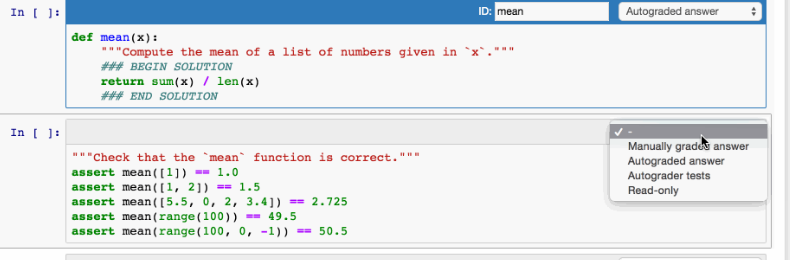
\includegraphics[width=0.8\textwidth]{img/nbgrader}
    \caption{Assigmenents in nbgrader system. Taken from \url{https://github.com/jupyter/nbgrader}.\label{fig:nbgrader}}
\end{figure}